%!TEX root = ../thesis.tex

\chapter[introduction]{Introduction}\label{chp:introduction}
%s
% SIZE: ~9 pages
%
% OUTLINE: Broad introduction to the topic.
% - Motivate the reader.
% - Why should they care about this topic? 
% - What is the historical context of decision-support, what are the practical implications of it, and what happens when it fails.

In an era where technology increasingly intertwines with healthcare, artificial intelligence is on the verge of becoming part of standard medical practice. 
Growing administrative burdens, rapid scientific progress in medicine, and aging populations have created a need to rethink how medical professionals are best enabled to successfully do their job. 
The application of artificial intelligence in medical decision-making, particularly in diagnosing and recommending treatments, is likely to hold significant potential for improving patient outcomes by reducing the effect of these issues. 
However, this prospect also raises concerns related to the reliability of such models as their decisions impact critical aspects of human health and well-being.

\todo[inline]{Can we find a better example than the Rhind Papyrus, or an additional one? It could be more on-point with decision-making and more well-known. Ideally, weave in an example of a failure of such technology.}
The evolution of technology to support and automate decision-making can be traced back to the development of algorithms and mathematical techniques by ancient civilizations. 
One example is the Egyptian Rhind Mathematical Papyrus, dated around 1550 BCE. It contains various mathematical techniques for calculations involving as multiplication, division, and fractions which were used for practical purposes like measuring land, constructing buildings, and sharing resources \cite{georges_universal_2001}. 
Around the same time, the Babylonians had developed a sophisticated system of mathematics, including algorithms for solving quadratic equations, calculating areas of shapes, and numerical methods for approximating square roots \cite{fowler_square_1998}. 

However, these new computing tools also brought new challenges. The Babylonian system of mathematics did not formalize the difference between rational and irrational numbers often leading to approximation errors and the common practice of approximating $\pi$ with 3. Apart from limitations inherent to the tools, inadequate human proficiency in their use was also a source of error. The Plimpton 322 clay tablet, for instance, contains several errors presumably made by a novice in Babylonian mathematics (\cref{fig:plimpton_332}) \cite{britton_plimpton_2011}. 
It is easy to forget that the challenges we face today in adopting new technologies are not new but have been faced by humans for thousands of years. Even in ancient times, it was important to understand the limitations of technology and the need for human expertise in using it.

\begin{figure}[t]
    \centering
    
\includegraphics[width=0.90\textwidth]{plimpton_322.png}
    \caption{Technology is difficult. The scribe of the Plimpton 322 clay tablet ($\sim$1800 BCE) made several errors when listing Pythagorean triplets, presumably struggling to grapple with Babylonian mathematics.}
    \label{fig:plimpton_332}
\end{figure}

While the quest to ease human decision-making has been ongoing for thousands of years, it was not until 1642 that the first mechanical calculator was successfully built by Blaise Pascal. 
And while the idea of a programmable computer with applications beyond pure arithmetic was first proposed by Ada Lovelace in 1843, 
it was not until the 1940s and 50s that % / 
% it took one-hundred years before / 
the first programmable, electronic, general-purpose digital computers were developed, starting with the ENIAC in 1945 (\cref{fig:eniac_programmers}) \cite{georges_universal_2001}. 
As they became more accessible, general-purpose computers were adopted widely across society for various applications in science and industry, including healthcare.
The societal changes brought about by the widespread adoption of computer technology through the latter half of the 20th century were so profound that some scholars refer to the era as the information age \cite{georges_universal_2001, harari_sapiens_2011}.
\todo[inline]{Expand on the history of modern computing.}

\begin{figure}[t]
    \centering
    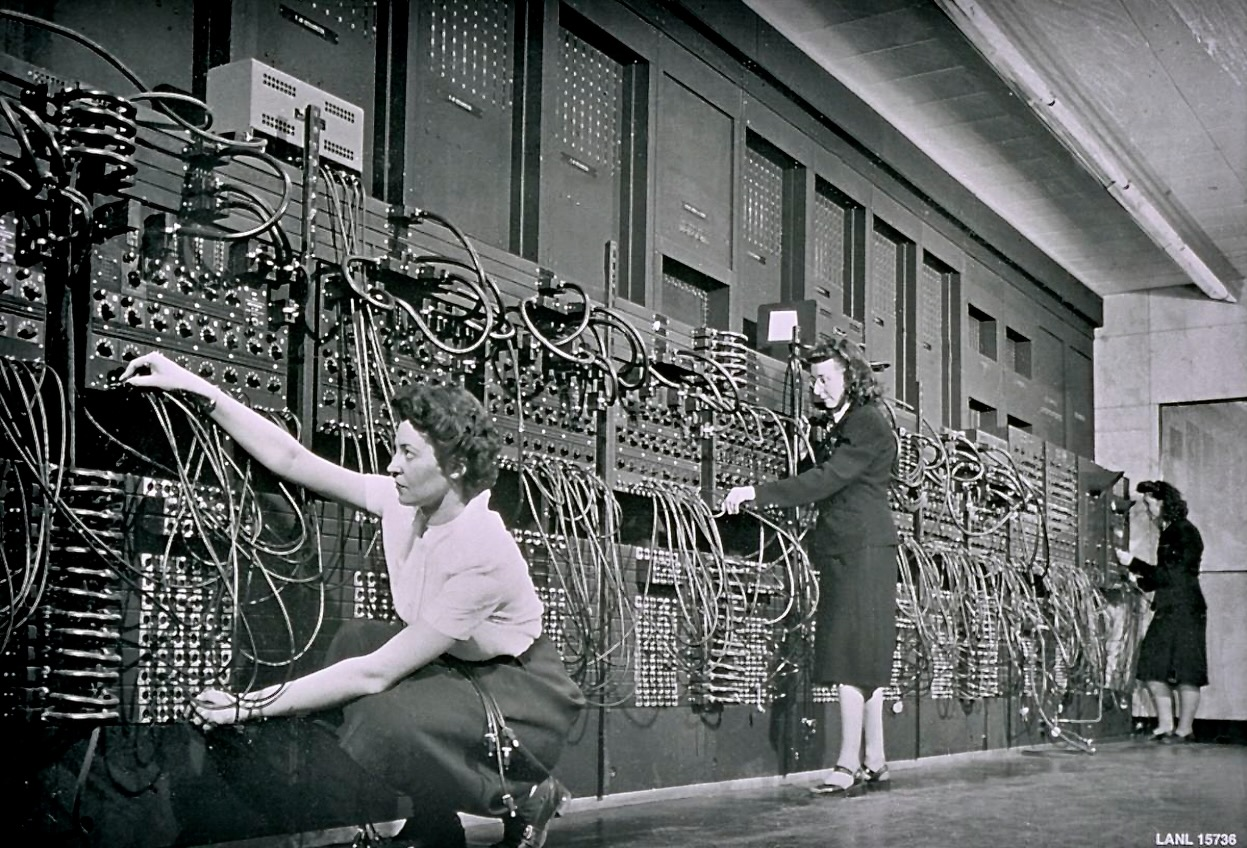
\includegraphics[width=0.95\textwidth]{eniac_programmers.jpeg}
    \caption{Ruth Lichterman (left) and Marlyn Wescoff (middle) were two of the female programmers of the ENIAC.} %Photo: \copyright Corbis/ Getty Images.}
    \label{fig:eniac_programmers}
\end{figure}

With the advent of the internet and the widespread adoption of digital technologies, the amount of data available to decision-makers has grown exponentially. 
This has led to a surge of interest in the scientific field of machine learning, a subfield of artificial intelligence that focuses on developing algorithms that can learn from data to recognize salient patterns and make predictions to guide decisions. 
Enabled by a massive increase in the power and availability of parallel computing resources, such methods have set new standards for the performance of computer systems in various domains, including speech recognition, computer vision, and natural language processing \cite{lecun_deep_2015}. 
In recent years, machine learning has also been applied within healthcare, where it has shown promising results in tasks such as medical imaging \cite{lundervold_overview_2019}, drug discovery \cite{chen_rise_2018}, and clinical decision support \cite{cite15, cite14}. 

However, these technologies come with the same risks as previous generations did, and in some cases, they may exacerbate them. 
Inherent limitations of the technology itself, human error, and the complexity of the real world are all factors that can lead to failures. A pertinent example is the nascent use of machine learning in autonomous driving systems: 
In 2018, the first incident of a self-driving car killing a pedestrian took place in Tempe, Arizona. 
The car, an SUV operated by Uber, was driving in autonomous mode when it struck a pedestrian crossing the street with her bicycle. 
According to the investigation by the National Transportation Safety Board, the car's sensors detected the pedestrian $5.6$ seconds before the crash, but it did not correctly predict her path or reduce the SUV's speed (\cref{fig:uber_nhsa_accident}). 
Specifically, during those seconds, the system incorrectly classified the pedestrian more than ten times, first as a vehicle, then as an unknown object and ultimately as a bicyclist, each time changing, or resetting, the predicted path. 
About one second before the crash, the system determined that a collision was imminent, but the situation exceeded the constraints within which the autonomous driving system was allowed to operate, and the car's safety driver failed to intervene \cite{nationaltransportationsafetyboardnhsa_collision_2019}. 

\begin{figure}[t]
    \centering
    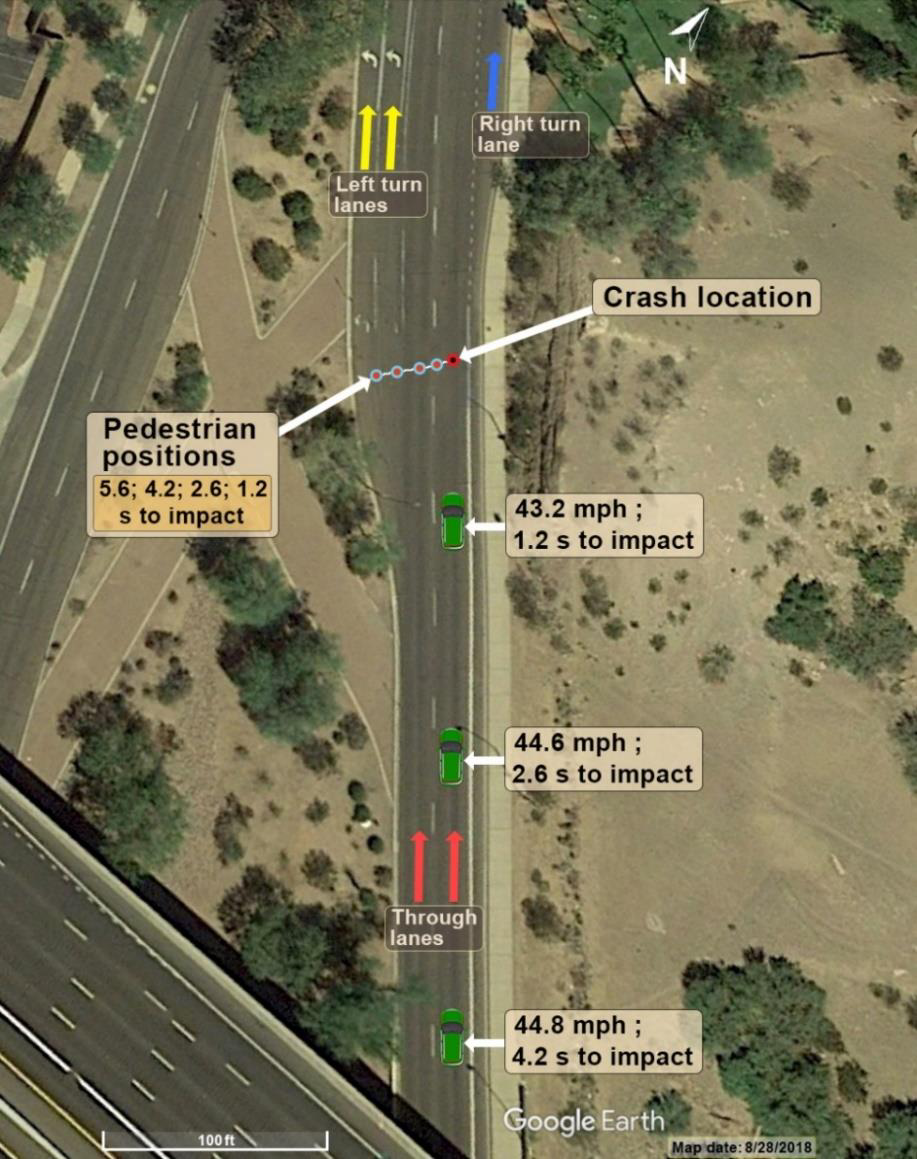
\includegraphics[width=0.95\textwidth]{uber_nhsa_accident.png}
    \caption{A pedestrian was killed by an Uber self-driving car in Tempe, Arizona in 2018. The car's sensors detected the pedestrian $5.6$ seconds before the crash, but the self-driving system failed to recognize the uncertainty of multiple object misclassifications and so did not correctly predict her path or reduce the SUV's speed \cite{nationaltransportationsafetyboardnhsa_collision_2019}.}
    % \caption{Aerial view of crash location showing path of pedestrian as she attempted to cross N. Mill Avenue and movement and speed of SUV at three points before impact. Pedestrian's path shows her position from initial detection ($5.6$ seconds before impact) until impact; SUV's position is shown at corresponding times beginning $4.2$ seconds before impact \cite{nationaltransportationsafetyboardnhsa_collision_2019}.}
    \label{fig:uber_nhsa_accident}
\end{figure}

Though this incident is an extreme one, it highlights the challenges of applying machine learning in real-world scenarios and underlines the need for machine learning systems to be robust to adverse or difficult situations.
Recently, European policymakers proposed a set of requirements for applications of machine learning to ensure that they are safe, reliable, and trustworthy \cite{europeancommission_briefing_2021}. This AI Act groups applications into three categories based on the potential risk they pose to society: limited risk, high risk, and unacceptable risk. Limited risk applications, for instance within gaming, must meet transparency requirements, and unacceptable risk applications, such as public use of facial recognition, are banned. High risk applications include those in healthcare and must meet a strict set of requirements focusing on anti-discrimination and robustness. 
%
One of the key ways to improve the safety, reliability and trustworthiness of machine learning systems is to equip them with the ability accurately estimate the uncertainty of their predictions. 
A model that can accurately estimate the uncertainty of its predictions can communicate to other systems or humans when it is unsure about a prediction, and so avoid making potentially catastrophic mistakes.
Fittingly, a recent study by the European Parliamentary Research Services concluded: 

\begin{center}

\textit{"Future AI solutions for healthcare should be implemented by integrating uncertainty estimation, a relatively new field of research that aims to provide clinicians with clinically useful indications on the degree of confidence in AI predictions"} \cite{europeanparliament_artificial_2022}. 

\end{center}

% \todo[inline]{Add something here about probability theory, Bayesian modelling etc. as a warm-up for potential solutions.}

\vspace{1em}
\begin{center}
\noindent\rule{0.2\textwidth}{0.5pt}
\end{center}
\vspace{1em}

% OUTLINE: Primer overview of the thesis. What are the topics and what is the context of the research.
\noindent The research presented in this thesis will focus on the use of machine learning in relation to uncertainty estimation, speech processing, and medical conversations. 
The research project of this thesis was formulated and carried out in collaboration with the Danish company Corti, which develops computer software for medical decision support. 
In the rest of this chapter, we will provide a high-level introduction to these topics and discuss the motivation behind the research project.


\section{Motivation and Corti's use-cases}
%
% OUTLINE: Motivate the research project. 
% - What is the context of the research and why is it important? 
% - What are the current applications of machine learning in the domain (decision-support in healthcare)?
% - What are the practical implications of the research? 
% - What are the challenges and limitations of the current state-of-the-art?
%
At the start of this project in 2020, Corti's main product was a software system providing decision-support for emergency medical dispatchers which operate the 1-1-2 emergency line in Copenhagen, Denmark and the 9-1-1 emergency line in Seattle, Washington in the United States.
The system, having been further developed, is still in use in 2023, and provides an interface for navigating a graph-based protocol, defined by the local emergency medical services, which dispatchers use to triage patients during emergency calls. 
Calls are transcribed in real-time using customer-domain automatic speech recognition and the system makes suggestions for the dispatcher to use in the conversation with the caller, including notifications about forgotten protocol questions \cite{havtorn_multiqt_2020} and potential cases of cardiac arrests \cite{cite15, cite14}. The system logs the details about the call and the dispatcher's actions to be used for later review and quality assurance. 


\subsection{Stroke recognition in emergency calls}
%
In 2021, Corti entered a research collaboration with the Capital Region of Denmark and the Copenhagen Emergency Services to develop a system for recognizing stroke cases in calls to the 1-1-2 emergency line and the 1813 medical helpline. 
Stroke is one of the biggest causes of disability and death worldwide \cite{cite1,cite2,cite3} and effective treatment is highly time-sensitive \cite{cite4,cite5}. The most common gateway to specialized treatment and hospital admittance is through prehospital telehealth services like emergency medical call centers, nurse advice call lines, and out-of-hours health services \cite{cite6,cite7}, however, studies have found that approximately half of all patients with stroke do not receive the correct triage for their condition from call-takers \cite{cite10,cite11,cite12}. 
This is likely due to the complexity of stroke cases which exhibit a wide range of symptoms that can be difficult to recognize over the phone. Additionally, out of total call volume, stroke cases are relatively rare, occurring in only $0.25\%$ of all calls to the Copenhagen 1-1-2 emergency line in 2021. This makes it difficult for call-takers to gain practical experience in recognizing stroke cases which exacerbates the general difficulty of recognizing the cases in the first place. Although several efforts have been made to improve the recognition of stroke cases in emergency calls \cite{cite13,cite14,cite15}, there is still a need for better tools to support call-takers in recognizing stroke cases.

A reasonable machine learning pipeline to assist in recognizing stroke on calls to emergency services might consist of an automatic speech recognition model to transcribe the conversation and a binary classifier to estimate the probability that what the transcript describes is a case of stroke. 
Such a system might be trained on a dataset calls with verified stroke and non-stroke cases and evaluated against a held-out test set of calls where the call-taker has indicated that they suspect a stroke. Due to the low prevalence of stroke cases, the dataset would likely be imbalanced, and the number of stroke cases limited. 
% The performance of such a system would depend on the quality of the automatic speech recognition model, the quality of the classifier, and the quality of the data used to train them. 
In such a system, many factors can lead to classification errors, and when that happens, we would like the model to express high degree of uncertainty. 
The automatic speech recognition model might be make an error in the transcription of particular word or phrase due to a noisy environment, overlapping, slurred or mumbling speech, or words not in the model's training data. 
The classifier might misclassify a conversation due to medically ambiguous symptoms, a general lack of information in the conversation, or errors of the speech recognizer propagated via the transcription. 
How to best make such models accurately represent and estimate the uncertainty of given predictions, and how to use it to improve the value of such a system, especially in cooperation with the call taker, is an open question.
What is clear, however, is that the ability of such a system to accurately estimate the uncertainty of given predictions is crucial for its safe and reliable deployment in the real world. Underconfident predictions could lead to unnecessary delays in treatment and increased costs for the healthcare system. Overconfident predictions could lead to misdiagnoses and potentially fatal consequences for patients.


\subsection{Medical coding of clinical notes}
%
During the course of the project presented in this thesis, Corti's product portfolio has expanded to include several new products. 
One of these is a software system for medical coding of clinical notes. 
When a patient is admitted to a hospital, the medical staff will write a clinical note describing the patient's diagnosis and the procedures they underwent, which includes drug prescriptions. 
These notes are then used for billing and reimbursement purposes, as well as for research and quality assurance. 
The clinical notes are written in natural language adhering to a certain structure, usually by a doctor. Later, a medical coder will assign a set of medical codes to the note based on its content. 
The process of medical coding is time-consuming and error-prone due to the number and complexity of medical diagnoses and procedures. For instance, the widely used International Classification of Diseases (ICD) standard consist of 55,000 medical codes in version 10 and 85,000 in version 11 \cite{worldhealthorganisationwho_international_2023}. Additionally, a single medical note will usually contain several diagnoses and procedures which must all be inferred from the clinical note. In public benchmarking datasets such as MIMIC-III and IV the number is around 15. Official guidelines describe how to code specific diagnoses and procedures and combinations thereof \cite{centersformedicaremedicaidservicesus_icd10cm_2023}. 
For instance, a code may have several exclusion or inclusion criteria which define when certain other codes must be coded along with it, or when they must not. 

\todo[inline]{
Discuss the role of uncertainty estimation in medical coding. 
Special challenges include significant class imbalance that cannot be removed by stratification since each example is associated with multiple labels.
Mutually dependent classes also complicates uncertainty estimation. Some classes are mutually exclusive, while others are not. Some classes are easily confused with each other. Uncertainty can be helpful in identifying code candidates as uncertain codes may need human review.
}

Many codes are rarely used and datasets for medical coding usually have a considerable class-imbalance which can be impossible to exactly correct for by stratified sampling since each example is associated with multiple labels. 

\todo[inline]{Write paragraph on using machine learning for medical coding and the role of uncertainty estimation in that.}




\section{Machine learning reliability}
%
Many modern machine learning models are deep neural networks with millions or even billions of parameters. 
These models are often referred to as black-box models as it is difficult to understand how they arrive at their predictions. 
The lack of interpretability makes it difficult to assess the reliability of the model's predictions. 
Furthermore, a number of factors, including the ability of deep neural networks to overfit, or even memorize, the training data \cite{arpit_closer_2017, burg_memorization_2021}, and the use of training objectives that are proxies for the evaluation metrics of interest, lead to models that often are miscalibrated; that is, the probability of a class predicted by the model does not reflect the true probability of the predicted class under the circumstances \cite{guo_calibration_2017, kull_temperature_2019}. Usually, the predicted probabilities are too extreme which leads to overconfident predictions. This means a model will often assign a high probability to the predicted class, even when it is wrong. 
In practice, such a model can be hard to trust. No model is perfect, but the inability to judge the certainty of a model's predictions makes it difficult to know how to weigh the model's predictions in a decision-making process. 

A connection can be made back to the incident with the Uber self-driving car. 
The multitude of rapid misclassifications made by the Uber self-driving car in Tempe is likely an indication that the model responsible for object-classification was overconfident in its predictions and unable to represent or communicate uncertainty to other systems in the car, or the safety driver. Instead, the model's predictions were taken at face value and subsystems in the car acted on them without appropriate consideration to their reliability.   


\subsection{Model calibration}

\todo[inline]{
    Expand in this discussion of overconfidence and calibration. E.g.: Calibration is fairly well understood in the context of classification, especially binary, but is harder in structured prediction such as automated speech recognition. Also: 
    Even if a model is well-calibrated, it can still be overconfident in wrong predictions - this is a problem in particular for rare events or adverse examples that were not presented to the model during training. Such examples are sometimes called out-of-distribution examples with reference to the training distribution. 
    For instance, a model trained to classify images of cats and dogs may have been well-calibrated, but if it is presented with an image of a horse, it has no option but to assign 100\% total probability to the cat and dog categories, even though that is clearly wrong. 
    Worse yet, we might expect the model to then at least assign 50\% probability to each of the cat and dog categories, but that behavior is not guaranteed. Specifically, since no horses were in the training data, the model will assign arbitrary probabilities to either class and so still risks being confidently wrong.
}

\subsection{Understanding uncertainty}
% 
% OUTLINE: Introduce aleatoric and epistemic uncertainty. 
% - Discuss the distinction between them and how they relate to the problem of uncertainty estimation in machine learning.
% - 
% 
%
The distinction in uncertainty estimation between known and unknown unknowns is sometimes referred to in terms of \textit{aleatoric uncertainty} and \textit{epistemic uncertainty} \cite{kendall_what_2017}. Both categories of uncertainty are usually used to describe uncertainties in a model's predictions or the model itself including its parameters, but they differ in their sources. 
Aleatoric uncertainty (from latin (aleatorius) 'dice player' or 'gambler') refers to uncertainty in the data itself due to true randomness which is irreducible even with infinite data. 
Epistemic uncertainty (from Greek (epistḗmē) 'knowledge') refers to uncertainty due to things one could in principle know but does not in practice. 
% It could arise because a measurement is not accurate, because the model neglects certain effects, or because particular data have been deliberately hidden. 
Epistemic uncertainty is sometimes referred to as \textit{systematic uncertainty} and aleatoric uncertainty as \textit{stochastic uncertainty} \cite{kendall_what_2017}. 
%, or, \textit{reducible} and \textit{irreducible} uncertainty, respectively. This latter terminology is somewhat misleading since epistemic uncertainty might not be reducible by additional data collection if the model is not sufficiently expressive to represent the data distribution, and aleatoric uncertainty is not necessarily irreducible if we can reduce inherent noise by improving the instruments used to collect the data \cite{kendall_what_2017}. 
Although the distinction between aleatoric and epistemic uncertainty is important, it is not always useful. For instance, a model may be uncertain about a particular prediction due to any of these two kinds of uncertainty. For that reason, the quantity of interest is usually the ``total" uncertainty, often referred to as \textit{predictive uncertainty}, which is simply the combined epistemic and aleatoric uncertainties. 

An example of aleatoric uncertainty is the uncertainty in the transcription of a word due to a noisy environment, overlapping, slurred or mumbling speech. We can reduce this uncertainty by improving the automatic speech recognition model, but we cannot eliminate it completely. 

Words not present in the training data are arguably sources of epistemic uncertainty although a good speech recognition model may generalize well to unseen words if its spelling and pronunciation follow the same patterns as the words in the training data. 

A stronger example of epistemic uncertainty is the occurrence of truly out-of-distribution examples, such as the horse in the image classifier example above: inputs unlike anything the model has seen during training that potentially require outputs unavailable to the model. 
In high-dimensional data with a practically unlimited diversity in possible out-of-distribution examples, it is impossible to collect enough data to eliminate epistemic uncertainty. If we included some horses in the training data, the model would likely be able to recognize them, but it would still be unable to recognize giraffes, or zebras, or unicorns. 
Ultimately, any practical machine learning model will have at least some sources of epistemic uncertainty i.e. unknown sources of uncertainty. 

% Aleatory uncertainty is often pretty straightforward to model since it is available in the data. Epistemic is much harder since we don't know much about it, other than we have only examples of where it is low.

% In real life applications, both kinds of uncertainties are present. Uncertainty quantification intends to explicitly express both types of uncertainty separately. The quantification for the aleatoric uncertainties can be relatively straightforward, where traditional (frequentist) probability is the most basic form. Techniques such as the Monte Carlo method are frequently used. A probability distribution can be represented by its moments (in the Gaussian case, the mean and covariance suffice, although, in general, even knowledge of all moments to arbitrarily high order still does not specify the distribution function uniquely), or more recently, by techniques such as Karhunen–Loève and polynomial chaos expansions. To evaluate epistemic uncertainties, the efforts are made to understand the (lack of) knowledge of the system, process or mechanism. Epistemic uncertainty is generally understood through the lens of Bayesian probability, where probabilities are interpreted as indicating how certain a rational person could be regarding a specific claim.

% In mathematics, uncertainty is often characterized in terms of a probability distribution. From that perspective, epistemic uncertainty means not being certain what the relevant probability distribution is, and aleatoric uncertainty means not being certain what a random sample drawn from a probability distribution will be.

\todo[inline]{Wrap this up. How to model aleatoric and epistemic uncertainty. Why do we care most about epistemic uncertainty (because we care about correctly estimating predictive uncertainty, and aleatoric is easy to model).}


\section{Scope of the thesis}
%
% OUTLINE: 
% - Tie together the different topics of the thesis and point briefly to the relevant papers.
%
The complete set of research published as part of this project covers a number of topics related to decision-support in medical conversations. 
One group of the produced studies is concerned with generative latent variable models and their applications to uncertainty estimation and speech modelling \cite{havtorn_hierarchical_2021,havtorn_benchmarking_2022,bergamin_modelagnostic_2022}. 
Another group of studies is concerned with self-supervised speech representation learning and automatic speech recognition \cite{borgholt_scaling_2021,borgholt_we_2021,mohamed_selfsupervised_2022,borgholt_brief_2022}. 
A final group deals with applications of machine learning within the medical domain, including recognition of stroke cases in calls to medical helplines \cite{wenstrup_retrospective_2023} and medical coding of clinical notes \cite{edin_automated_2023}. 

This first part of the thesis ties together these different studies by providing a high-level overview of the research topic and summarizing the main contributions of the thesis.









\iffalse


Uncertainty is a fundamental part of human experience. The ability to understand and quantify uncertainty is crucial in making informed decisions, drawing meaningful conclusions, and assessing the reliability of predictions made from observations. Yet, capturing this ability in a mathematical model is a difficult task. 

Uncertainty estimation has long been a central topic in the field of statistics. It has traditionally been addressed through methods like confidence intervals, hypothesis testing, and Bayesian inference. Confidence intervals provide a range of plausible values for a parameter, while hypothesis testing evaluates the significance of differences between groups or variables \cite{blitzstein_introduction_2019}. Bayesian inference, on the other hand, offers a powerful framework to incorporate prior knowledge and update beliefs based on observed data using probability theory. These approaches have been extensively studied and applied in various domains, from social sciences to natural sciences, to improve the robustness and generalizability of statistical analyses \cite{gelman_bayesian_2013}. However, the widespread adoption in diverse applications of machine learning, and in particular deep neural networks, has posed new challenges in dealing with uncertainty. 

Machine learning algorithms are designed to learn patterns from data and make predictions or decisions based on those patterns. Since many applications of machine learning are concerned with real-world phenomena, it is important to understand the uncertainty associated with the predictions made by such a model. For instance, in medical diagnosis, knowing the uncertainty in a model's prediction is crucial when the consequences of a false positive or false negative can be significant. In speech recognition, knowing that a certain word was hard to transcribe for the model can help avoid misinterpretation of the transcribed text.


% The performance of machine learning models is highly dependent on the quality and quantity of data used for training. In many cases, the data used to train machine learning models are collected from the real world, and therefore, may contain biases and errors which models may learn to mirror. In addition, the complexity of modern machine learning models makes it difficult to understand how they arrive at their predictions. This is especially true for deep neural networks, which are often referred to as black-box models. The lack of interpretability makes it difficult to assess the reliability of the model's predictions.

% Modern speech processing relies on high-performance parallel computing [40, 157], large volumes of data [136, 213], and years of innovation in model design [109, 266].

% 40: High performance convolutional neural networks for document processing \cite{chellapilla_high_2006}
% 157: Imagenet classification with deep convolutional neural networks \cite{krizhevsky_imagenet_2012}
% 136: Libri-light: A benchmark for asr with limited or no supervision \cite{kahn_libri-light_2020}
% 213: Librispeech: an ASR corpus based on public domain audio books \cite{panayotov_librispeech_2015}
% 109:  Long short-term memory \cite{hochreiter_long_1997}
% 266: Attention Is All You Need \cite{vaswani_attention_2017}


\section{Machine learning and societal risk}
\todo[inline]{Discuss the role of uncertainty aware models in the context of risk.}
\cite{europeancommission_briefing_2021}


\section{Motivation: Speech recognition}


\section{Motivation: Automated medical coding}


\subsection{Uncertainty in machine learning}

\todo[inline]{Revise this section with less focus on individual methods and more focus on overall trends.}

In the context of machine learning, uncertainty is often represented by a probability distribution. The most common approach is to use Bayesian methods, where uncertainty is captured by posterior distributions over model parameters and predictions \cite{gelman_bayesian_2013}. Bayesian neural networks, for instance, offer a powerful framework to model uncertainty in deep learning architectures \cite{neal_bayesian_1995}. By incorporating prior beliefs and updating them based on observed data, these networks can produce probabilistic predictions that provide a measure of uncertainty. This is particularly useful in applications where high-confidence predictions are required, and the consequences of errors can be significant.

Recently, another interesting approach to uncertainty estimation in machine learning is the use of Monte Carlo Dropout \cite{gal_dropout_2016}. Monte Carlo Dropout leverages the idea of dropout regularization, originally employed during training to prevent overfitting. To form a prediction with associated uncertainty, Monte Carlo Dropout proposes to make multiple forward passes through the network while sampling different dropout masks for each one. This leads to obtaining a distribution of outputs for each input sample and the variance among these sampled predictions serves as a measure of uncertainty. It is computationally efficient and can be easily incorporated into existing deep learning architectures, making it an attractive choice for uncertainty estimation.

Furthermore, there has been an interest in ensemble methods for uncertainty estimation \cite{lakshminarayanan_simple_2017}. Ensembles combine the predictions of multiple models to obtain a more robust and calibrated uncertainty measure. Bagging and boosting techniques, which have been widely used in the field of statistics, have found their way into the realm of machine learning for uncertainty estimation as well. By training multiple models with different initialization or using diverse learning algorithms, ensembles can capture different sources of uncertainty, thereby providing a comprehensive assessment of the overall uncertainty in the predictions.

% We compare our framework with several major related lines of work. First, our work focuses on the quantification of epistemic uncertainty, which refers to the errors coming from the inadequacy of the model or data noises. This is different from aleatoric uncertainty, which refers to the intrinsic stochasticity of the problem [87, 91, 112, 59, 34], or predictive uncertainty which captures the sum of epistemic and aleatoric uncertainties (but not their dissection) [89, 92, 12, 3, 22]. Regarding epistemic uncertainty, a related line of study is deep ensemble that aggregates predictions from multiple independent training replications [76, 70, 38, 8, 89]. This approach, as we will make clear later, can reduce and potentially quantify procedural variability, but a naive use would require demanding retraining effort and does not address data variability. Another line is the Bayesian UQ approach on neural networks [41, 2]. This regards network weights as parameters subject to common priors such as Gaussian. Because of the computation difficulties in exact inference, an array of studies investigate efficient approximate inference approaches to estimate the posteriors [40, 46, 16, 31, 30, 90, 74, 53]. While powerful, these approaches nonetheless possess inference error that could be hard to quantify, and ultimately finding rigorous guarantees on the performance of these approximate posteriors remains open to our best knowledge.

% 87: 
% 91: 
% 112:
% 59: 
% 34: 

% 89: 
% 92: 
% 12:
% 3: 
% 22: 

% 76: 
% 70: 
% 38: 
% 8: 
% 89: X

% 41: 
% 2: 

% 40:
% 46:
% 16:
% 31:
% 30:
% 90:
% 74:
% 53:




\iffalse

General challenges in uncertainty estimation:
\begin{enumerate}
    \item \textbf{Accuracy}: The uncertainty estimation method should be accurate.
    \item \textbf{Interpretability}: The uncertainty estimation method should be interpretable.
    \item \textbf{Robustness}: The uncertainty estimation method should be robust to adversarial attacks.
    \item \textbf{Applicability}: The uncertainty estimation method should be applicable to a wide range of models without requiring extensive modifications.
    \item \textbf{Efficiency}: The uncertainty estimation method should be computationally efficient at training and prediction time.
    \item \textbf{Scalability}: The uncertainty estimation method should scale to large datasets.
\end{enumerate}







Uncertainty is a fundamental part of human experience. Yet, capturing it in a mathematical model is a difficult task. Historically, uncertainty estimation has been a central topic in the field of statistics. While classical statistical methods have provided valuable insights, they often assume well-defined probability distributions and may not fully capture the complexities of uncertainty in real-world scenarios. Moreover, they tend to rely heavily on parametric assumptions, which might not hold true for complex data with high-dimensional features and non-linear relationships. Therefore, in recent years, researchers have turned their attention towards more flexible and data-driven approaches to model uncertainty in various domains.

In the field of machine learning, uncertainty is often represented by a probability distribution. The most common approach is to use Bayesian methods, where uncertainty is captured by posterior distributions over model parameters and predictions. Bayesian neural networks, for instance, offer a powerful framework to model uncertainty in deep learning architectures. By incorporating prior beliefs and updating them based on observed data, these networks can produce probabilistic predictions that provide a measure of uncertainty. This is particularly useful in applications where high-confidence predictions are required, and the consequences of errors can be significant.

Recently, another promising approach to uncertainty estimation in machine learning is the use of Monte Carlo Dropout (MC Dropout). MC Dropout leverages the idea of dropout regularization, originally employed during training to prevent overfitting. During prediction, MC Dropout takes multiple forward passes through the network with dropout enabled, which leads to obtaining a distribution of outputs for each input sample. The variance among these sampled predictions serves as a measure of uncertainty. MC Dropout has shown remarkable success in various tasks such as image classification, object detection, and natural language processing. It is computationally efficient and can be easily incorporated into existing deep learning architectures, making it an attractive choice for uncertainty estimation.

Furthermore, there has been a surge of interest in ensemble methods for uncertainty estimation. Ensembles combine the predictions of multiple models to obtain a more robust and calibrated uncertainty measure. Bagging and boosting techniques, which have been widely used in the field of statistics, have found their way into the realm of machine learning for uncertainty estimation as well. By training multiple models with different initializations or using diverse learning algorithms, ensembles can capture different sources of uncertainty, thereby providing a comprehensive assessment of the overall uncertainty in the predictions.

Despite the progress made in uncertainty estimation for machine learning models, challenges still remain. One key concern is the interpretability of uncertainty measures. While probabilistic outputs are more informative than point estimates, effectively communicating uncertainty to end-users and decision-makers is not trivial. Developing visualization techniques and intuitive explanations for uncertainty is an ongoing area of research. Additionally, quantifying uncertainty in high-dimensional data or complex models with massive amounts of parameters requires careful consideration and efficient computational strategies.

In conclusion, uncertainty estimation is a crucial aspect of machine learning models, enabling them to make more informed and reliable predictions. Researchers continue to explore innovative techniques to better represent and quantify uncertainty, allowing for safer and more trustworthy deployment of machine learning systems in real-world scenarios.





Uncertainty is a fundamental part of human experience. Yet, capturing it in a mathematical model is a difficult task. Historically, uncertainty estimation has been a central topic in the field of statistics. Understanding and quantifying uncertainty is crucial in making informed decisions, drawing meaningful conclusions, and assessing the reliability of predictions and inferences derived from data.


In the field of statistics, uncertainty is traditionally addressed through methods like confidence intervals, hypothesis testing, and Bayesian inference. Confidence intervals provide a range of plausible values for a parameter, while hypothesis testing evaluates the significance of differences between groups or variables. Bayesian inference, on the other hand, offers a powerful framework to incorporate prior knowledge and update beliefs based on observed data using probability theory. These approaches have been extensively studied and applied in various domains, from social sciences to natural sciences, to improve the robustness and generalizability of statistical analyses.
However, the advent of machine learning and its widespread adoption in diverse applications has posed new challenges and opportunities in dealing with uncertainty. 

Machine learning algorithms are designed to learn patterns from data and make predictions or decisions based on that knowledge. In many cases, it is not enough to provide a single deterministic prediction; it is equally important to convey the level of uncertainty associated with the prediction. For instance, in medical diagnosis, knowing the uncertainty in a model's prediction is crucial when the consequences of a false positive or false negative can be significant. In autonomous driving systems, understanding uncertainty becomes essential to ensure the safety of passengers and pedestrians.

To address the uncertainty challenge in machine learning, researchers have developed various techniques to represent and quantify uncertainty. One of the common approaches is the use of probabilistic models, where uncertainty is captured in the form of probability distributions. Instead of providing a single point prediction, probabilistic models generate a range of possible outcomes along with their associated probabilities. Bayesian neural networks, Gaussian processes, and variational autoencoders are some examples of such models that have gained prominence in the quest for uncertainty-aware machine learning.

Another avenue for dealing with uncertainty in machine learning is through ensemble methods. Ensemble learning combines multiple models to improve predictive accuracy and can also provide uncertainty estimates. By aggregating the outputs of diverse models, ensemble methods can identify situations where predictions are consistent among the models, leading to higher confidence, and cases where the models disagree, indicating higher uncertainty.

As the intersection of statistics and machine learning grows increasingly important, the integration of these two domains has become an active area of research. The incorporation of probabilistic modeling and Bayesian approaches into machine learning methods opens up new possibilities for developing more robust, interpretable, and calibrated models. Moreover, the synergy of statistical techniques with deep learning, reinforcement learning, and other advanced machine learning paradigms has the potential to push the boundaries of uncertainty quantification and application even further.

In this thesis, we aim to explore and contribute to the field of uncertainty in statistics and machine learning. We will investigate state-of-the-art methods for uncertainty estimation, delve into their theoretical underpinnings, and evaluate their performance in various real-world scenarios. By gaining a deeper understanding of uncertainty and its implications, we aspire to pave the way for more reliable, trustworthy, and accountable AI systems in the future.

In the following chapters, we will begin by reviewing the relevant literature on uncertainty in both statistics and machine learning, providing a comprehensive overview of the current landscape. We will then present our proposed methodologies and empirical studies, illustrating how uncertainty quantification can enhance decision-making processes and mitigate risks in practical applications. Finally, we will conclude with a discussion of our findings, potential limitations, and future research directions in this exciting and rapidly evolving field.

\fi
\fi